\section{Caracterización del sensor}
Una de las actividades principales dentro de la pruebas del sistema es realizar la caracterización de nuestro sensor de flujo, caudalimetro.
Para dicha actividad, se realizaron una serie de pruebas unitarias, las cuáles en conjunto, nos brindan la capacidad de conocer el comportamiento
real y no solo teorico de nuestro sensor.

Dicho comportamiento será modelado puede ser modelado a partir de una función, la cuál, se encuentra dentro del datasheet del sensor solicitado.

\begin{equation}
F = 4.8 * Q
\end{equation}

\paragraph{Fórmula para la caracterización}
La fórmula anterior nos permite conocer la frecuencia de flujo de nuestro sensor. Estos pulsos serán recibidos por nuestra aplicación móvil dentro de la cual se realizará la conversión necesaria para conocer los litros ingresados a nuestro automóvil.\\
La fórmula, consta de una incógnita multiplicada por un factor de conversión, 
dicha incógnita representa el número de litros por minuto que pasan a través del sensor, el factor de conversión fué determinado por el fabricante.

\begin{figure}[H]
	\centering
	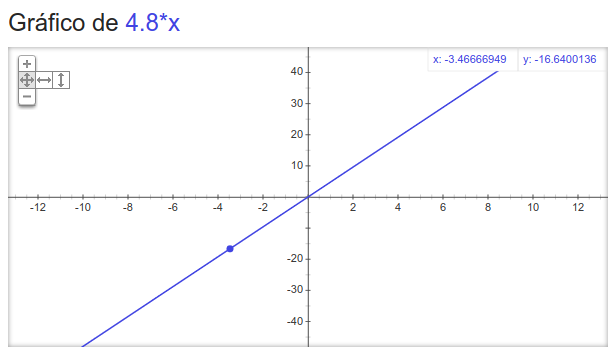
\includegraphics[width=.7\textwidth]{Capitulo6/caracterizacion/img/FormulaSensor.png}
	\caption{Gráfica de la Frecuencia de flujo del caudalimetro utilizado}
\end{figure}

La gŕafica anterior muestra una correspondencia lineal entre el número de litros ingresado y la frecuencia de flujo de salida, por lo que se puede inferir un comportamiento proporcional al variar la cantidad de litros ingresados.

\paragraph{Caractarización a partir de pulsos}
La salida del sensor entrega una señal de pulsos cuadrados cuya frecuencia corresponde al flujo del líquido modelado por la fórmula anterior, dicho tren de pulsos es provocado por la apertura y cierre del interruptor de muestreo a intervalos regulares. En esta ocasión la apertura y cierre del interruptor se da mediante la creación de un pulso magnético generado mediante el Efecto Hall.
Debido a el tren de pulsos generado es modelado por la fórmula anterior, podemos inferir que la cantidad de pulsos generados tendrán de igual forma una correspondencia lineal con el número de litros ingresados a nuestro sistema.


\paragraph{Tratamiento del tren de pulsos}
Como ya se mencionó en secciones previas, el tren de pulsos es enviado nuestra aplicación móvil partir de un sensor bluetooth. Dentro de nuestra aplicación, se realiza la suma total de los pulsos, a continuación se describe la fórmula empleada dentro de la aplicación para convertir el tren de pulso en litros.

\begin{equation}
\sum_{pulso \neg 0}^{ pulso = 0} frecuenciaFlujo / (4.8 * 60) = litrosTotales
\end{equation}

La fórmula anterior indica como los pulsos pertenecientes al tren serán sumados y posteriormente divididos entre el tiempo total multiplicado por la constante de amortiguamiento del sensor, al depender directamente de un fenómeno con un comportamiento lineal (el tren de pulsos) y al ser multiplicado por una constante, se puede decir que la salida será un fenómeno lineal de igual forma.

\paragraph{Caracterización de la medición}
Como ya observamos, todos los fenómenos que se encuentran inmersos desde la medición del sensor hasta el cálculo de los litros en la aplicación tienen un comportamiento lineal. De esta forma podemos tomar la entrada del primer fenómeno y la salida del último y verificar esa correspondencia. La primer entrada será la cantidad de litros que sabemos se deben ingresar, y la última salida será la cantidad de litros medidos. Para estas pruebas se realizó la siguiente tabla.

\begin{figure}[H]
	\centering
	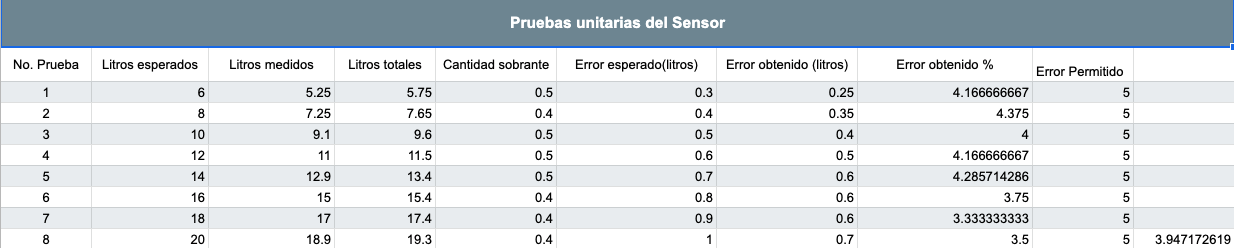
\includegraphics[width=1\textwidth]{Capitulo6/caracterizacion/img/Tabla.png}
	\caption{Tabla pruebas de caracterización}
\end{figure}
La tabla anterior fue graficada para poder observar el comportamiento de los datos, y corroborar si nuestro sistema de medición en efecto tiene un comportamiento lineal.

\begin{figure}[H]
	\centering
	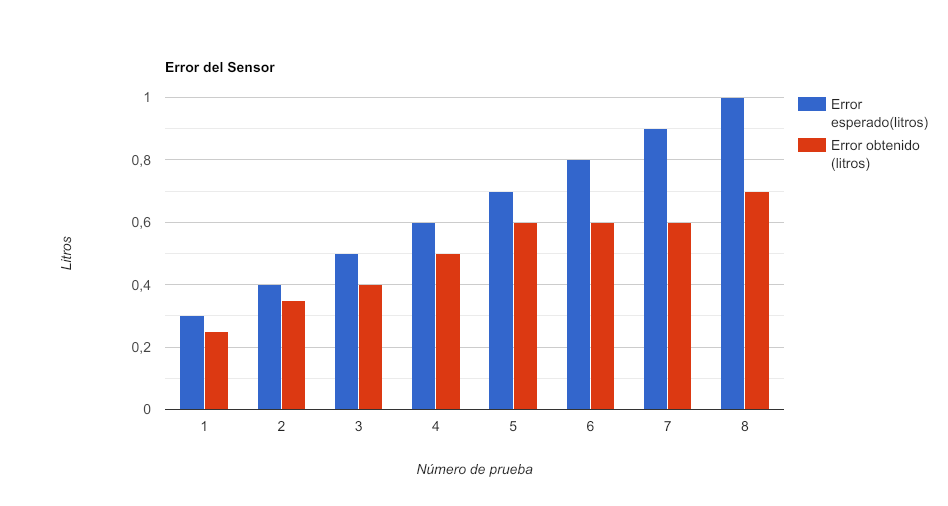
\includegraphics[width=1\textwidth]{Capitulo6/caracterizacion/img/Error_sensor.png}
	\caption{Mediciones obtenidas a partir de los experimentos}
\end{figure}

La gráfica anterior nos permite observar las diferencias que hubo en cuanto a las salidas esperadas y las salidas obtenidas dentro del proceso de medición, dichos datos claramente muestran un comportamiento lineal, además se permite observar el error obtenido. Los mismos datos, serán representados con otro tipo de gráfico para apreciar de mejor forma el comportamiento lineal.

\begin{figure}[H]
	\centering
	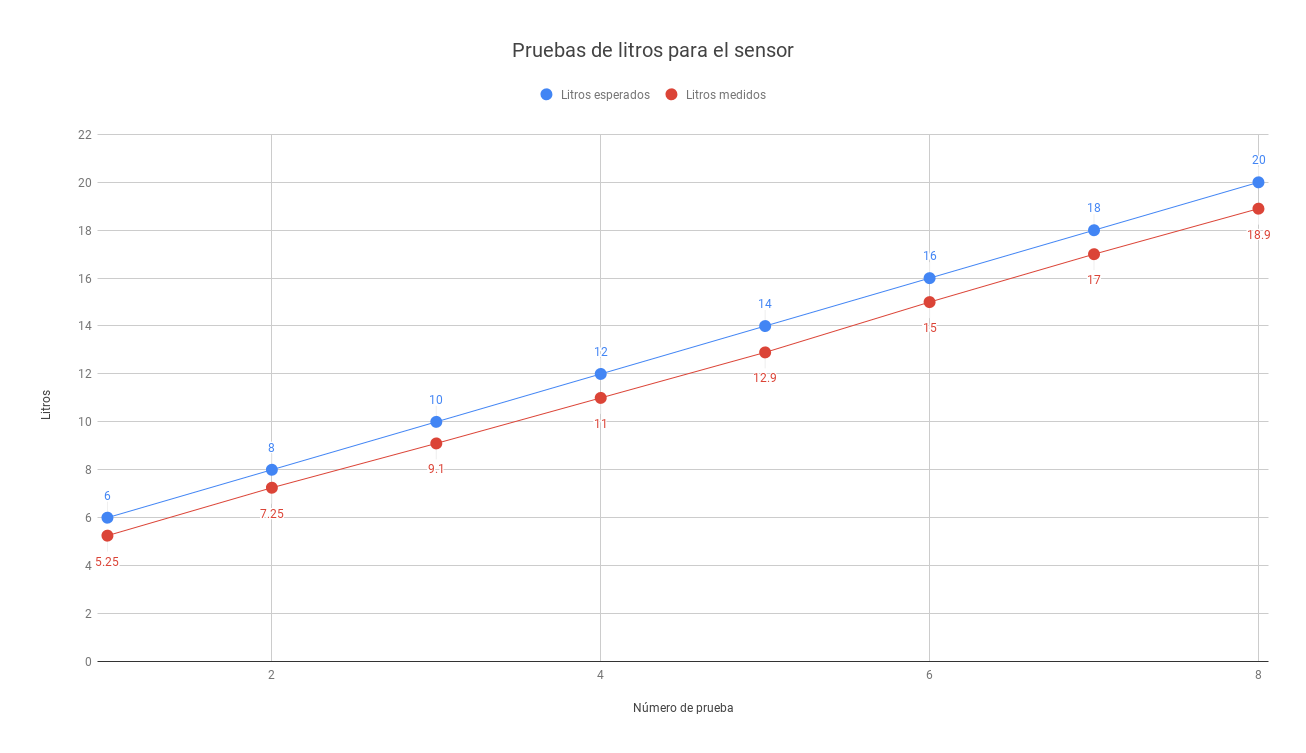
\includegraphics[width=1\textwidth]{Capitulo6/caracterizacion/img/Pruebas-de-litros-para-el-sensor}
	\caption{Comportamiento lineal de los datos de medición}
\end{figure}

La gráfica anterior permite demostrar que todas las variables involucradas dentro de nuestra medición tienen un comportamiento linear. Los litros esperados tienen una variación de 2 litros por prueba, lo que genera una gráfica lineal con una pendiente positiva.

Finalmente analizaremos una variable importante dentro de la caracterización de nuestro sensor y es la del error. Según el datasheet de nuestro sensor, así como la Norma Oficial para la regulación de instrumentos de medición, una dispensador de líquido de combustible puede tener hasta un 5 por ciento de error.

Podemos observar en la Figura 6.8 Pruebas Unitarias del Sensor que nuestro sensor posee un error del 3.9 por ciento, el cuaĺ se encuentra debajo del límite establecido por la Norma.

A continuación, se anexa una gráfica donde podemos notar que incluso la gráfica del error de nota un comportamiento lineal.

\begin{figure}[H]
	\centering
	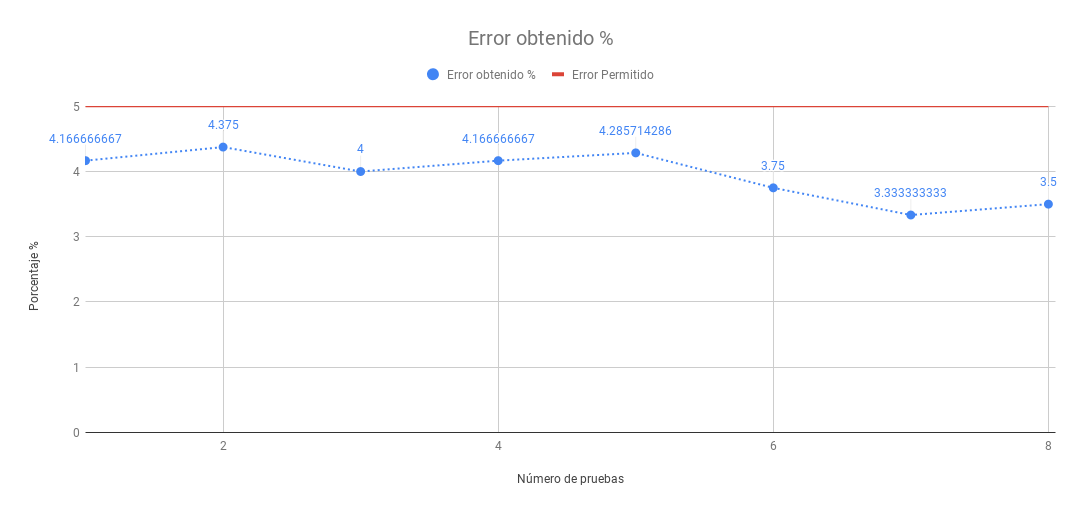
\includegraphics[width=1\textwidth]{Capitulo6/caracterizacion/img/Error_porcentaje.png}
	\caption{Error de medición durante las pruebas}
\end{figure}

\paragraph{Caracterización final}Finalmente, podemos concluir que nuestro sensor tiene un comportamiento de tipo lineal tanto en la parte teórica como en la práctica, posee una salida con un tren de pulsos por lo que no fué necesario realizar algún tratamiento a la señal resultante para poder trabajar de manera discreta. La caracterización de un sensor  con siste en el cálculo  de la ecuación característica de su comportamiento. Dicha ecuación, fué proporcionada por el fabricante y comprobada de manera práctica mediante nuestra pruebas.